\documentclass[numeric]{anvil-paper}
\usepackage{tikz}
\usepackage{pgfplots}
\usepgfplotslibrary{groupplots}
\pgfplotsset{compat=1.17}
\usetikzlibrary{positioning}

\newcommand{\F}{\mathbb{F}}
\newcommand{\code}[1]{\texttt{#1}}
\newtheorem{proposition}{Proposition}

\title{Parity Words and Grid Shares:\\ Error-Correcting Mnemonics and Secret Sharing\\ over the BIP39 Wordlist}
\author{Robb Walters}
\date{November 2026}

\begin{document}
\maketitle

\begin{abstract}
A secret that no vendor can reset has to be copied onto paper or metal by hand
and read back years later. BIP39 mnemonics detect a copying mistake but cannot
repair one, and splitting a secret with Shamir's scheme multiplies the number of
hand-copied artefacts while giving each only a detection checksum. We observe
that a BIP39 word is already one symbol of the field with 2048 elements, and put
both error correction and threshold sharing in that field. A phrase with $k$
appended Reed--Solomon \emph{parity words} recovers from $e$ wrong and $s$
unreadable words whenever $2e+s\le k$, and from swapped, dropped and extra words
by a small edit search; the original mnemonic is unchanged. Sharing such phrases
word by word gives \emph{grid shares}: any $t$ of $n$ cards recover the secret,
fewer reveal nothing, every card repairs itself, and spare cards repair each
other. Across 28{,}000 fault-injection trials of a Lean~4 implementation the
combined decoder never returned a wrong secret. With all cards of a 3-of-5 set
at hand it recovered 99.7\% of secrets when one word in ten was wrong, where
per-card repair recovered 36\% and per-card checksums none.
\end{abstract}

\section{Introduction}
\label{sec:intro}

Shares of a secret can repair themselves and each other, at the level where
people make mistakes: whole words. That is the claim of this paper. It rests on
one observation. The BIP39 wordlist~\citep{bip39} has $2048 = 2^{11}$ entries,
so a written word is one element of the finite field $\F_{2^{11}}$, and both
tools a backup format needs are linear algebra over a field. Reed--Solomon
codes~\citep{reed1960polynomial} add redundancy within one written phrase.
Shamir's scheme~\citep{shamir1979how} spreads a secret over several phrases.
When both use the same field and the same symbols, they compose into a product
code, and the result is decoded as one object.

The problem is practical. A 256-bit key with no reset path must be stored in
full, by its owner, for years. In a controlled study, 40\% of participants could
not reproduce an assigned 12-word BIP39 phrase after three days and 49\% could
not after seven; of 41 failures examined, 14 were one wrong word or one wrong
word plus two words out of order~\citep{ambati2026notall}. BIP39's checksum
(4 bits for 12 words, 8 for 24) says that such a phrase is wrong and nothing
about where. Splitting the secret makes this worse: a 3-of-5 sharing has five
phrases to copy, and deployed formats check each share separately
(Section~\ref{sec:related}).

Our contributions:
\begin{itemize}
\item \textbf{Parity words} (Section~\ref{sec:parity}). An $N{+}k$ format: $N$
  BIP39 words followed by $k$ words of Reed--Solomon parity over $\F_{2^{11}}$.
  The first $N$ words are an unmodified mnemonic. A repair procedure handles
  wrong, unreadable, swapped, dropped and extra words and reports ambiguity
  instead of guessing.
\item \textbf{Grid shares} (Section~\ref{sec:grid}). Shamir sharing applied word
  by word to parity phrases. Each card is a valid parity phrase; each word
  position across cards is a Shamir sharing; the two are decoded together.
\item \textbf{A hidden header and a digest.} A card's number and threshold ride
  in a codeword symbol that is never printed, and two words of a hash of the
  secret give the non-linear check that no linear code can supply.
\item \textbf{Measurements} (Section~\ref{sec:experiments}) from a 900-line
  Lean~4 implementation~\citep{moura2021lean}, and worked custody arrangements
  (Section~\ref{sec:scenarios}).
\end{itemize}
The ingredients are inherited: Reed--Solomon codes, Shamir sharing, product
codes and hash checks are all decades old. New is their arrangement on the BIP39
alphabet, the unprinted header, and a decoder that refuses instead of guessing.
We give no formal proofs of the implementation and no handwriting data; word
error rates are parameters of the experiments
(Section~\ref{sec:limits}).

\section{Related Work}
\label{sec:related}

\paragraph{Mnemonic formats.}
BIP39~\citep{bip39} appends a truncated SHA-256 checksum to the entropy before
cutting it into 11-bit words; the check detects errors only. Polyseed
\citep{polyseed} uses one Reed--Solomon check word over a 2048-element field in
a 16-word phrase, enough to detect a wrong word or fill in one missing word.
Our single-phrase format generalises that idea to any $k$ and keeps the BIP39
phrase as a prefix.

\paragraph{Shared mnemonics.}
SLIP39~\citep{slip39} shares a secret bytewise over $\F_{2^8}$ and protects each
share with a three-word RS1024 checksum that its specification uses for
detection. codex32~\citep{bip93} is closest in spirit: shares are bech32 strings
with a BCH checksum that corrects up to four character substitutions, and the
checksum is linear, so shares derived by interpolation stay valid. codex32's
alphabet is single characters and its checksum is applied per share; it does
not decode across shares. Our cards use dictionary words, which resist
transcription slips better than character strings, and add the joint decoding.

\paragraph{Sharing and coding.}
\citet{mceliece1981sharing} showed that the shares of Shamir's scheme form a
Reed--Solomon codeword, so $m$ shares tolerate $\lfloor (m-t)/2\rfloor$ wrong
ones. \citet{tompa1989how} showed that a participant who lies about a share can
steer the reconstruction undetected and added a check to the secret; our digest
plays that role against accidents. Spreading one long codeword among parties
without fresh randomness is a ramp scheme~\citep{blakley2007security,
franklin1992communication}; Section~\ref{sec:ramp} quantifies why that is unsafe
here. Product codes go back to \citet{elias1954error}, and decoding several
Reed--Solomon words that share error positions is studied as interleaved
Reed--Solomon decoding~\citep{schmidt2009collaborative}. The redundancy
arithmetic is that of RAID~\citep{patterson1988case}: the first two parity
words are the P and Q blocks of a RAID-6 stripe.

\section{Parity Words}
\label{sec:parity}

\subsection{The code}

Let $\F=\F_{2^{11}}$ be built with the primitive polynomial $x^{11}+x^2+1$, and
let $\alpha$ be the class of $x$, a generator of the multiplicative group of
order 2047. A word with index $w\in\{0,\dots,2047\}$ in the BIP39 list is the
field element whose bits are $w$.

A protected phrase is $c=(c_0,\dots,c_{n-1})$ with $n=N+k\le 2047$: $N$ data
words followed by $k$ parity words. It is valid when its $k$ \emph{syndromes}
vanish:
\begin{equation}
S_j(c)=\sum_{p=0}^{n-1} c_p\,\alpha^{pj}=0,\qquad j=0,\dots,k-1 .
\label{eq:syn}
\end{equation}
$S_0$ is the exclusive-or of all words and $S_1$ weights each word by its
position. The valid phrases form a Reed--Solomon code with minimum distance
$k+1$~\citep{reed1960polynomial}: any two valid phrases differ in at least $k+1$
positions. Hence the standard guarantee: if $e$ words are wrong and $s$ are
known to be missing or unreadable, the original is the unique valid phrase
within reach whenever
\begin{equation}
2e+s\le k .
\label{eq:cap}
\end{equation}
Encoding is systematic. The parity words are the unique values that satisfy
\eqref{eq:syn} given the data words, found by treating the $k$ parity positions
as erasures. The data words are untouched, so if they are a BIP39 mnemonic any
existing wallet reads the first $N$ words and ignores the rest.

Decoding uses the Euclidean key-equation solver of \citet{sugiyama1975method},
a search over positions for the error locations, and the error-value formula of
\citet{forney1965decoding}. A decoding is accepted only if the corrected phrase
satisfies~\eqref{eq:syn} and \eqref{eq:cap}.

\subsection{Repair beyond substitutions}

People do not only substitute words. They exchange two, skip one, or copy one
twice. These are not symbol errors: a dropped word shifts every later word to a
wrong position. The repair procedure therefore enumerates \emph{edit
hypotheses} and lets the code judge each:
\begin{itemize}
\item \emph{As written}: decode with up to $\lfloor k/2\rfloor$ substitutions.
\item \emph{Swap}: exchange any two positions, then decode. A swap leaves $S_0$
  unchanged and there are $n(n-1)/2$ of them, so a swap may be combined with
  at most $\lfloor (k-2)/2\rfloor$ further substitutions.
\item \emph{Dropped words} (phrase short by $d\le 3$): insert $d$ erasures at
  every choice of positions, then decode.
\item \emph{Extra words} (phrase long by $d\le 3$): delete every choice of $d$
  words, then decode.
\end{itemize}
Each surviving candidate has a cost: the number of edits plus substitutions.
The procedure returns \emph{all} candidates of minimum cost. One candidate is a
repair; several are reported as ambiguous, and the user chooses or finds a
better copy. When the data words have a BIP39 length their SHA-256 checksum is
applied as a second, independent filter before the minimum is taken.

The restriction on swaps matters. Without it, a 24+2 phrase with two wrong
words was ``repaired'' to a different valid phrase in 97.6\% of trials during
development, because some swap plus one substitution nearly always lands on a
codeword.

\section{Grid Shares}
\label{sec:grid}

\subsection{Construction}

Fix a threshold $t$, a number of cards $n\le 31$, and $k$. Let the \emph{secret
row} $r_0\in\F^{W}$ be a valid phrase of width $W=N+k$ whose data words are the
seed followed by $d$ digest words (below). Draw $t-1$ further rows
$r_1,\dots,r_{t-1}$ with uniformly random data words and their own parity. Card
$i\in\{1,\dots,n\}$ is, word by word,
\begin{equation}
y_i = r_0 + x_i\,r_1 + x_i^2\,r_2+\dots+x_i^{t-1}r_{t-1},
\qquad x_i = \text{the field element with bit pattern } i .
\label{eq:card}
\end{equation}
Figure~\ref{fig:grid} shows the arrangement.

\begin{figure}[tb]
\centering
% Grid shares diagram (t = 2, n = 3)
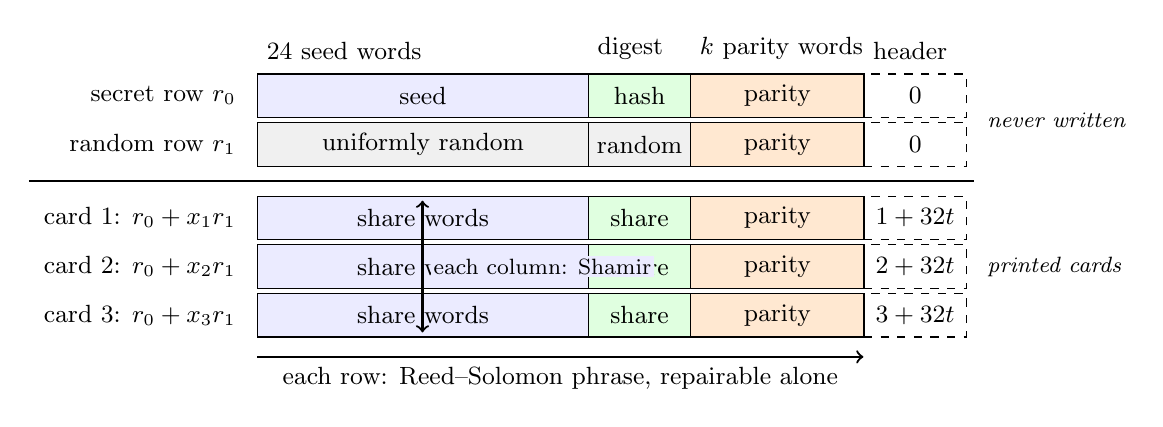
\begin{tikzpicture}[x=1cm,y=0.62cm,font=\small,
  cell/.style={draw,minimum height=0.55cm,inner sep=1pt,anchor=west},
  data/.style={cell,minimum width=4.2cm,fill=blue!8},
  dig/.style={cell,minimum width=1.3cm,fill=green!12},
  par/.style={cell,minimum width=2.2cm,fill=orange!18},
  hdr/.style={cell,minimum width=1.3cm,dashed}]
\node[anchor=south west] at (0,0.55) {24 seed words};
\node[anchor=south west] at (4.2,0.55) {digest};
\node[anchor=south west] at (5.5,0.55) {$k$ parity words};
\node[anchor=south west] at (7.7,0.55) {header};
% hidden rows
\node[anchor=east] at (-0.15,0) {secret row $r_0$};
\node[data] at (0,0) {seed};
\node[dig] at (4.2,0) {hash};
\node[par] at (5.5,0) {parity};
\node[hdr] at (7.7,0) {0};
\node[anchor=east] at (-0.15,-1) {random row $r_1$};
\node[data,fill=gray!12] at (0,-1) {uniformly random};
\node[dig,fill=gray!12] at (4.2,-1) {random};
\node[par] at (5.5,-1) {parity};
\node[hdr] at (7.7,-1) {0};
\draw[thick] (-2.9,-1.75) -- (9.1,-1.75);
\node[anchor=west,font=\footnotesize\itshape] at (9.15,-0.5) {never written};
\node[anchor=west,font=\footnotesize\itshape] at (9.15,-3.5) {printed cards};
% cards
\foreach \i/\y in {1/-2.5,2/-3.5,3/-4.5}{
  \node[anchor=east] at (-0.15,\y) {card \i: $r_0 + x_{\i} r_1$};
  \node[data] at (0,\y) {share words};
  \node[dig] at (4.2,\y) {share};
  \node[par] at (5.5,\y) {parity};
  \node[hdr] at (7.7,\y) {$\i+32t$};
}
% row arrow
\draw[->,thick] (0,-5.35) -- (7.7,-5.35) node[midway,below] {each row: Reed--Solomon phrase, repairable alone};
% column arrow
\draw[<->,thick] (2.1,-2.15) -- (2.1,-4.85);
\node[anchor=west,font=\footnotesize,fill=blue!8,inner sep=1pt] at (2.2,-3.5) {each column: Shamir};
\end{tikzpicture}

\caption{Grid shares for $t=2$, $n=3$. Each printed card (a row) is a valid
parity phrase, so it can be repaired alone. Each word position (a column) is a
Shamir sharing, so any $t$ cards determine it and spare cards expose a wrong
entry. The header symbol is part of every card's codeword but is never
printed.}
\label{fig:grid}
\end{figure}

\begin{proposition}
\label{prop:grid}
(a) Every card $y_i$ satisfies~\eqref{eq:syn}.
(b) Any $t$ cards determine $r_0$.
(c) Any $t-1$ cards are statistically independent of the data words of $r_0$.
(d) The cards of any $m\ge t$ holders, read as an $m\times W$ array, differ
between two distinct dealings in at least $(k+1)(m-t+1)$ entries.
\end{proposition}

\begin{proof}
(a) The syndromes are linear and each $r_d$ has zero syndromes.
(b) In each column the card values are evaluations of a polynomial of degree
below $t$ at distinct points; interpolation at $0$ gives the column of $r_0$.
(c) In each data column this is Shamir's scheme~\citep{shamir1979how}, with
independent randomness per column; the parity words of a card are a function
of its data words and add nothing.
(d) The array is a codeword of the product of a length-$m$ Reed--Solomon code
of distance $m-t+1$~\citep{mceliece1981sharing} with the row code of distance
$k+1$; distances of a product multiply~\citep{elias1954error}.
\end{proof}

Part (d) bounds what any decoder can promise: up to
$\lfloor((k+1)(m-t+1)-1)/2\rfloor$ wrong words \emph{anywhere} among the $m$
cards leave the dealing uniquely determined. For 30-word cards with $k=4$ that
is 2 words with two cards of a 2-of-3 set, 4 with all three, and 7 with all
five cards of a 3-of-5 set. Our decoder (Section~\ref{sec:decoder}) is iterative
and is not shown to reach this bound in every pattern; in exchange it handles
bursts far beyond it.

\subsection{The unprinted header}

A card must say which evaluation point it belongs to, and a number written in a
corner is one more thing to smudge. We extend every card's codeword by one
symbol at position $W$, after the last printed word, holding
$h_i = i + 32t$. The printed parity words are computed over the data words and
this header. Because the code is linear, the header's contribution to the
parity words is $h_i$ times a fixed vector, which the decoder subtracts before
working on columns.

If the card's number is legible, the header is known and the card keeps its
full strength. If it is not, the header is one more erasure; when that leaves
too little parity, the decoder tries each of the 31 possible numbers as if
known and keeps the one that brings the card within reach. The header costs no
written words, and a card with the wrong number attached fails its own check.

\subsection{The digest}
\label{sec:digest}

A linear code cannot tell a correct reconstruction from a consistent wrong one.
With exactly $t$ cards, every combination of valid cards interpolates to
\emph{some} valid phrase, including when one card comes from a different
dealing. We therefore append $d$ \emph{digest words} to the seed before
sharing: the first $d$ 11-bit groups of
SHA-256(\code{"bip39-parity/digest"} $\|$ seed words as two bytes each).
A reconstruction is accepted only if its digest words match its seed words. A
wrong candidate passes with probability $2^{-11d}$; we use $d=2$. If the first
reconstruction fails the digest and more than $t$ cards repaired, the decoder
tries each $t$-subset and so identifies the card that does not belong.

The digest is shared like every other data word, so by
Proposition~\ref{prop:grid}(c) fewer than $t$ cards learn nothing about it. A
standard card is then 24 seed words, 2 digest words and $k$ parity words:
30 words for $k=4$.

\subsection{Decoding}
\label{sec:decoder}

\begin{enumerate}
\item \emph{Rows.} Repair each card alone as in Section~\ref{sec:parity}. A
  card that repairs uniquely is \emph{confirmed}. A card that does not, but
  whose number is known, is kept as unconfirmed evidence.
\item \emph{Columns.} For each word position, find the polynomial of degree
  below $t$ that agrees with the most cards, using confirmed cards alone when
  there are at least $t$. With exactly $t$ values the column is taken as given;
  with more, it is settled only if at least $t+1$ values agree and no rival
  polynomial ties.
\item \emph{Iterate.} Settled columns supply words to unconfirmed cards, which
  are then decoded again as rows; newly confirmed cards settle more columns.
\item \emph{Rescue.} If confirmed cards are one short of $t$, guess the error
  positions on an unconfirmed card, erase them, and accept the result only if
  every guessed position then agrees with another card.
\item \emph{Check.} Interpolate the secret row, verify its syndromes and its
  digest, and fall back to $t$-subsets as described above. If nothing passes,
  refuse.
\end{enumerate}

\subsection{Why not split one long phrase?}
\label{sec:ramp}

A tempting shortcut is to encode once with large $k$ and hand each party a
segment, since any $N$ of the $N+k$ words recover the rest. This is a ramp
scheme, not threshold sharing: with no fresh randomness, every word a party
holds is 11 bits of constraint on the secret. A party holding $h$ words of a
24-word secret faces $264-11h$ unknown bits, so a 12-word segment leaves 132
bits of the phrase, or 124 bits of entropy after the 8-bit BIP39 checksum.
Two colluding segment holders have everything. Grid shares cost longer cards
and give the property people expect from Shamir: below the threshold, nothing.

\section{Experiments}
\label{sec:experiments}

\subsection{Setup}

The implementation is about 900 lines of Lean~4 (toolchain 4.36.0), compiled
to native code through Lean's C backend, with no dependencies beyond the Lean
core library. Two harnesses inject faults: \code{tests} for single phrases and
\code{gridtests} for grids. Each trial draws fresh entropy, deals, damages the
written words, and decodes. An outcome is \emph{correct} (the original seed is
returned), \emph{wrong} (a different seed is returned), or \emph{refused}; for
single phrases, \emph{correct} means the original phrase is the single
candidate. The random generator is seeded with a fixed value, so every table is
reproduced exactly by the command given in Section~\ref{sec:repro}.

Grids use 24 seed words, 2 digest words and $k=4$ unless stated. A word error
replaces a word by a different uniformly random word, independently per word.
A \emph{burn} makes a run of consecutive words unreadable. A \emph{foreign}
card is the same-numbered card of an unrelated dealing; a \emph{garbage} card
is random words. We compare three ways of using the same cards:
\begin{itemize}
\item \emph{Checksum only}: a card counts only if it is exactly valid as
  written; the first $t$ such cards are interpolated. This models per-share
  detection.
\item \emph{Card parity}: each card is repaired alone; the first $t$ repaired
  cards are interpolated. This models per-share correction.
\item \emph{Grid}: the full decoder of Section~\ref{sec:decoder} with the
  digest.
\end{itemize}
With 400 trials a reported percentage has a 95\% confidence half-width of at
most 5 points; we do not interpret smaller differences.

\subsection{Single phrases}

Table~\ref{tab:single} gives the fraction of trials in which repair returned
exactly the original phrase. Everything inside the capacity~\eqref{eq:cap} is
repaired, as it must be. The interesting rows are the edits. Two parity words
repair a swap or a dropped word; three repair two dropped words or a wrong word
plus a dropped word; four repair any two wrong words. Without the BIP39
checksum as a filter, 24+2 leaves 13--15\% of swaps ambiguous (the right phrase
is among the candidates), and the one dangerous outcome, a single wrong
candidate, appeared only for faults beyond the capacity of $k=2$, in 0.5--1.5\%
of trials. With $k\ge 3$ it did not appear.

\begin{table}[tb]
\centering
\caption{Single phrases: percentage of 200 trials in which the original phrase
was the unique repair, using the BIP39 checksum as a filter. ``Refused'' means
no candidate was offered in any trial.}
\label{tab:single}
\small
\begin{tabular}{lcccccc}
\toprule
Fault & 12+2 & 12+3 & 12+4 & 24+2 & 24+3 & 24+4 \\
\midrule
1 wrong word & 100 & 100 & 100 & 100 & 100 & 100 \\
2 unreadable words & 100 & 100 & 100 & 100 & 100 & 100 \\
2 adjacent words swapped & 100 & 100 & 100 & 100 & 100 & 100 \\
any 2 words swapped & 100 & 100 & 100 & 99.5 & 100 & 100 \\
1 dropped word & 100 & 100 & 100 & 100 & 100 & 100 \\
1 extra word & 100 & 100 & 100 & 100 & 100 & 100 \\
2 dropped words & 1 & 99.5 & 100 & 30 & 100 & 100 \\
1 wrong + 1 dropped & refused & 99.5 & 100 & refused & 99.5 & 100 \\
2 wrong words & refused & refused & 100 & refused & refused & 100 \\
\bottomrule
\end{tabular}
\end{table}

\subsection{Grids}

Table~\ref{tab:grid} and Figure~\ref{fig:rates} give the main result. Three
things stand out.

\emph{Spare cards turn into error correction.} With all five cards of a 3-of-5
set and one word in ten wrong, the grid decoder recovers 99.7\% of secrets;
repairing cards one at a time recovers 36\%, because three of five cards must
each have at most two errors.

\emph{Bursts.} Five consecutive unreadable words exceed what $k=4$ can fill, so
no card repairs alone and both per-card methods recover nothing. The grid
decoder recovers 90\% (2-of-3) and 98.5\% (3-of-5), because the burns fall in
different columns on different cards.

\emph{Wrong cards.} When one card is from another dealing, per-card methods
return a wrong secret whenever that card is among the first $t$ used: 61--67\%
of trials. The grid decoder with digest returns the right secret every time
when a spare card exists and refuses every time when none does.

Across every grid experiment in this paper (28{,}000 trials) the grid decoder
with digest returned no wrong secret.

\begin{table}[tb]
\centering
\caption{Grid shares, 30-word cards ($k=4$), 400 trials per cell. Entries are
the percentage of trials that returned the correct secret, for 2-of-3 / 3-of-5.
A bracket gives the percentage that returned a \emph{wrong} secret where that
is not zero; the remainder were refused.}
\label{tab:grid}
\small
\begin{tabular}{lccc}
\toprule
Damage & Checksum only & Card parity & Grid \\
\midrule
\multicolumn{4}{l}{\emph{All $n$ cards at hand}}\\
1\% of words wrong & 80.7 / 88.2 & 100 / 100 & 100 / 100 \\
3\% of words wrong & 33.0 / 36.0 & 99.2 / 99.5 & 99.7 / 100 \\
5\% of words wrong & 12.7 / 3.7 & 93.5 / 96.2 & 96.7 / 100 \\
10\% of words wrong & 1.0 / 0.0 & 40.7 / 36.0 & 61.2 / 99.7 \\
5 words burnt on every card & 0 / 0 & 0 / 0 & 89.7 / 98.5 \\
8 words burnt on every card & 0 / 0 & 0 / 0 & 34.7 / 63.0 \\
one card is foreign & 33.0 / 39.0 [67 / 61] & 33.0 / 39.0 [67 / 61] & 100 / 100 \\
\midrule
\multicolumn{4}{l}{\emph{Only $t$ cards at hand}}\\
1\% of words wrong & 57.2 / 45.7 & 99.5 / 99.2 & 99.5 / 99.2 \\
3\% of words wrong & 16.7 / 6.2 & 87.7 / 79.0 & 87.7 / 79.0 \\
5\% of words wrong & 3.2 / 0.7 & 62.0 / 50.7 & 62.0 / 50.7 \\
one card is foreign & 0 / 0 [100 / 100] & 0 / 0 [100 / 100] & 0 / 0 \\
\bottomrule
\end{tabular}
\end{table}

\begin{figure}[tb]
\centering
% Correct recoveries vs per-word error rate; data: refs/experiments/grid-main-k4.txt
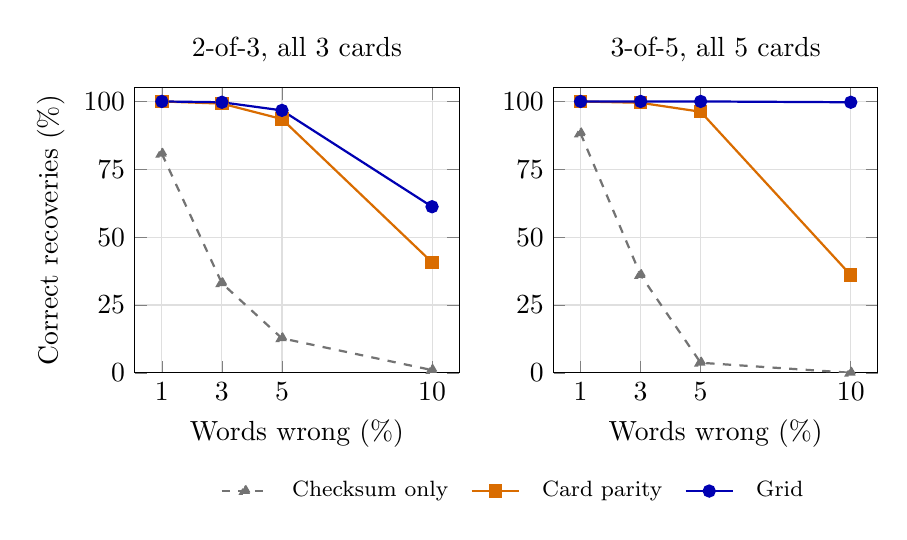
\begin{tikzpicture}
\begin{groupplot}[
  group style={group size=2 by 1, horizontal sep=1.2cm, ylabels at=edge left},
  width=0.47\linewidth, height=5.2cm,
  xlabel={Words wrong (\%)}, ylabel={Correct recoveries (\%)},
  xtick={1,3,5,10}, ymin=0, ymax=105, ytick={0,25,50,75,100},
  grid=major, grid style={gray!25},
  legend style={font=\footnotesize, draw=none, fill=none, legend columns=3, column sep=6pt, at={(-0.12,-0.34)}, anchor=north},
  every axis plot/.append style={thick, mark size=2pt}]
\nextgroupplot[title={2-of-3, all 3 cards}]
\addplot[color=black!55, mark=triangle*, dashed] coordinates {(1,80.7) (3,33.0) (5,12.7) (10,1.0)};
\addplot[color=orange!85!black, mark=square*] coordinates {(1,100) (3,99.2) (5,93.5) (10,40.7)};
\addplot[color=blue!70!black, mark=*] coordinates {(1,100) (3,99.7) (5,96.7) (10,61.2)};
\nextgroupplot[title={3-of-5, all 5 cards}]
\addplot[color=black!55, mark=triangle*, dashed] coordinates {(1,88.2) (3,36.0) (5,3.7) (10,0.0)};
\addlegendentry{Checksum only}
\addplot[color=orange!85!black, mark=square*] coordinates {(1,100) (3,99.5) (5,96.2) (10,36.0)};
\addlegendentry{Card parity}
\addplot[color=blue!70!black, mark=*] coordinates {(1,100) (3,100) (5,100) (10,99.7)};
\addlegendentry{Grid}
\end{groupplot}
\end{tikzpicture}

\caption{Correct recoveries with all cards at hand as the per-word error rate
grows (data of Table~\ref{tab:grid}, 400 trials per point). Joint decoding
gains little over per-card repair with one spare card (2-of-3) and nearly
removes the dependence on error rate with two (3-of-5).}
\label{fig:rates}
\end{figure}

\subsection{With exactly $t$ cards, only $k$ helps}

The lower half of Table~\ref{tab:grid} is the scheme's weak case. With exactly
$t$ cards there are no spare rows, the grid decoder equals per-card repair, and
\emph{every} card must repair. At 3\% wrong words, $k=4$ recovers 88\% (2-of-3)
and 79\% (3-of-5). Table~\ref{tab:k} shows that the remedy is more parity per
card: $k=8$ restores 99\% at the cost of four more written words.

\begin{table}[tb]
\centering
\caption{Only $t$ cards at hand: percentage correct for 2-of-3 / 3-of-5 as the
number of parity words per card grows ($k=4$: 400 trials; $k=6,8$: 300
trials). No trial returned a wrong secret.}
\label{tab:k}
\small
\begin{tabular}{lccc}
\toprule
Words wrong & $k=4$ (30 words) & $k=6$ (32 words) & $k=8$ (34 words) \\
\midrule
3\% & 87.7 / 79.0 & 95.6 / 95.0 & 99.0 / 99.6 \\
5\% & 62.0 / 50.7 & 83.6 / 78.0 & 95.6 / 91.6 \\
\bottomrule
\end{tabular}
\end{table}

\section{Custody Arrangements}
\label{sec:scenarios}

The number of cards a group can bring together decides which half of
Table~\ref{tab:grid} applies. Table~\ref{tab:scen} works through three
arrangements, with 250 trials per cell and $k=4$.

\begin{table}[tb]
\centering
\caption{Percentage of correct recoveries by number of cards brought together
($k=4$, 250 trials per cell, grid decoder with digest; no trial returned a
wrong secret). ``Foreign'' replaces one card by a card of another dealing and
``garbage'' by random words (with 1\% word errors on the rest); ``burnt'' is
five consecutive unreadable words on every card.}
\label{tab:scen}
\small
\begin{tabular}{llcccccc}
\toprule
Scheme & Cards & 1\% & 3\% & 5\% & Garbage & Foreign & Burnt \\
\midrule
3-of-6 & 3 & 99.2 & 82.4 & 50.8 & 0 & refused & 0 \\
       & 4 & 100 & 98.4 & 94.0 & 100 & 100 & 76.8 \\
       & 6 & 100 & 100 & 100 & 100 & 100 & 100 \\
\midrule
3-of-5 & 3 & 99.6 & 83.2 & 54.8 & 0 & refused & 0 \\
       & 4 & 100 & 98.8 & 89.6 & 99.6 & 100 & 72.0 \\
       & 5 & 100 & 100 & 100 & 100 & 100 & 98.0 \\
\midrule
4-of-9 & 4 & 98.4 & 73.6 & 40.0 & 0 & refused & 0 \\
       & 5 & 100 & 99.2 & 87.6 & 96.8 & 100 & 62.8 \\
\bottomrule
\end{tabular}
\end{table}

\paragraph{Three people, two cards each (3-of-6).}
One person holds two cards and learns nothing. Any two people hold four: one
more than the threshold, which is the ``4 cards'' row. The pair can lose or
ruin one card and still recover, can identify a card that does not belong, and
recover 98\% of the time at a 3\% word error rate. All three together are
insensitive to every fault we injected. The cost of the convenience is on the
theft side: one person plus any single stolen card reaches the threshold.

\paragraph{An owner with three cards and two backup holders (3-of-5).}
The owner can recover alone, but with exactly $t$ cards and therefore no
margin: 83\% at a 3\% error rate, and nothing if one card is lost or burnt. One
backup holder's card restores the margin (98.8\%). The two backup holders
together hold two cards and learn nothing. Since the owner's three cards are a
complete key, they should be stored in separate places, and an owner who
expects to recover alone should use $k=6$ or $k=8$ (Table~\ref{tab:k}).

\paragraph{Weighted inheritance (4-of-9).}
An owner holds four cards, an executor two, and three heirs one each. The owner
recovers alone; after the owner's death the executor and any two heirs reach
four, and with the third heir five. The heirs alone hold three and learn
nothing, and so does the executor alone. Weights come for free because cards
are interchangeable evaluations.

\paragraph{The general rule.}
Plan for one more card than the threshold to be present at recovery. A spare
card moves an arrangement from the lower half of Table~\ref{tab:grid} to the
upper half, and it is the only way to survive a card that is wrong as a whole.

\section{Discussion}
\label{sec:limits}

\paragraph{Security.}
Secrecy below the threshold is information-theoretic
(Proposition~\ref{prop:grid}c) and depends on the $t-1$ random rows being
uniform; the dealer must use a cryptographic random source. Parity and header
reveal nothing about the seed, but a single card does reveal the threshold and
its own number. The digest protects against accidents and against a holder who
alters a card without knowing the seed, who passes with probability $2^{-22}$.
It is not a defence against a dealer who cheats or a holder who already knows
the secret; verifiable secret sharing addresses those and is out of scope.
Redundancy does not help an attacker who has $t$ cards, and does not weaken the
seed: parity words are public functions of words the holder already has.

\paragraph{Limits of the evidence.}
(1) There are no published per-word error rates for handwritten word lists, so
the 1--10\% range is an assumption, and real errors are not uniform: people
confuse similar words, which a uniform model does not capture. (2) Faults
within a card were independent except for burns. (3) The implementation is
tested, not verified; its unit tests cover the field axioms, SHA-256 and BIP39
reference vectors, and decoding within capacity for $k=1,\dots,8$, but no
theorem about the decoder is proved in Lean. (4) The grid decoder is a
heuristic. It discards a card with dropped words that does not repair alone
instead of using it as evidence, and the rescue step applies only when
confirmed cards are one short. Proposition~\ref{prop:grid}(d) says a better
decoder exists for some patterns. (5) The edit search grows quickly; it is
bounded at three dropped or extra words.

\paragraph{Choosing $k$.}
The measurements suggest $k=4$ when a spare card will normally be present and
$k=6$ or more when recovery from exactly $t$ cards is the expected path. For an
unshared 24-word phrase, $k=3$ covers every single edit and $k=4$ any two wrong
words.

\paragraph{Open directions.}
A packed variant that shares two secret words per column would give 12-word
cards for a 24-word seed at the price of ramp-style leakage between one and
$t$ cards. Measuring real transcription errors would replace our assumed rates.
The Lean sources are a natural basis for a verified decoder.

\section{Reproducibility}
\label{sec:repro}

All numbers come from the accompanying source tree, built with \code{lake build}
under the Lean toolchain \code{v4.36.0}. The harness outputs are stored
verbatim with the paper sources in the folder \code{refs/experiments/}, each
headed by its command:
\begin{itemize}
\item Table~\ref{tab:single}: \code{lake exe tests 200}
\item Table~\ref{tab:grid} and Figure~\ref{fig:rates}:
  \code{lake exe gridtests 400}
\item Table~\ref{tab:k}: \code{lake exe gridtests 300 "only t cards," 6},
  and the same with \code{8}
\item Table~\ref{tab:scen}, one command per scheme:\\
  \code{lake exe gridtests custom 250 4 3 6 3 4 6}\\
  \code{lake exe gridtests custom 250 4 3 5 3 4 5}\\
  \code{lake exe gridtests custom 250 4 4 9 4 5}
\end{itemize}
The random seed is fixed in the harness (39). The command-line tool exposes
the scheme directly: the subcommands \code{encode}, \code{check} and
\code{repair} of \code{parity39} handle single phrases, and \code{split} and
\code{combine} handle grids.

\section{Conclusion}
\label{sec:conclusion}

Because a BIP39 word is a field element, a mnemonic can carry Reed--Solomon
parity in its own alphabet, and Shamir shares of such mnemonics are mnemonics
of the same kind. Two parity words repair a swap or a dropped word and four
repair any two wrong words. Shared as a grid, cards repair themselves and each
other: with a spare card the decoder survived burns and foreign cards that
defeat per-card checks, and in 28{,}000 trials it never returned a wrong
secret. With no spare card, reliability comes only from parity per card, and
the arrangement should be chosen with that in mind.

\bibliographystyle{plainnat}
\bibliography{refs}

\end{document}
